\documentclass{article}[12pt,a4paper]

%!TEX root = main.tex

\def\finex{{\unskip\nobreak\hfil
\penalty50\hskip1em\null\nobreak\hfil{\Large $\diamond$}
\parfillskip=0pt\finalhyphendemerits=0\endgraf}}

\newenvironment{lmref}[1]{%
	\vspace*{0.3cm}
	\noindent {\bf  Lemma #1.}}

\newenvironment{thref}[1]{%
	\vspace*{0.3cm}
	\noindent {\bf  Theorem #1.}}

\newenvironment{corref}[1]{%
	\vspace*{0.3cm}
	\noindent {\bf  Corollary #1.}}


\newcommand{\picalc}{$\pi$-calculus~}
\newcommand{\ms}[1]{\mathsf{#1}}
\newcommand{\ctx}{\mathtt{C}}
\newcommand{\co}[1]{\overline{#1}}
\newcommand{\proj}[1]{\mathtt{proj}(#1)}
\newcommand{\projs}[1]{\mathtt{proj_n}(#1)}
\newcommand{\lts}[1]{\xrightarrow{#1}}
\newcommand{\comm}[1]{\textcolor{blue}{#1}}
\newcommand{\red}[1]{\textcolor{red}{#1}}
\newcommand{\key}{\mathtt{keys}}
\newcommand{\flts}[1]{\overset{#1}\twoheadrightarrow}
\newcommand{\rev}{^{\bullet}}
%\newcommand{\forw}{_{\twoheadrightarrow}}
\newcommand{\eq}{\sim} 
\newcommand{\env}{\theta} 
\newcommand{\ex}{e} 
\newcommand{\proc}[3]{\langle #1,#2,#3\rangle } 
\newcommand{\erl}[1]{\hookrightarrow_{#1}} 
\newcommand{\mem}[2]{[#1\;;#2]}
\newcommand{\bl}[1]{\textcolor{blue}{#1}}
\newcommand{\rd}[1]{\textcolor{red}{#1}}
\newcommand{\mtt}[1]{\mathtt{#1}}
\newcommand{\pid}{\mathtt{pid}}
\newcommand{\procl}[4]{\langle #1,#2,#3,#4\rangle } 
\newcommand{\con}{\equiv}
\newcommand{\conk}{\equiv_k}
\newcommand{\extcon}{\equiv_c}
\newcommand{\de}{\delta}
\newcommand{\G}{\Gamma}
\newcommand{\logg}[1]{\rightharpoonup_{#1}}
\newcommand{\rlogg}[1]{\leftharpoondown_{#1}}
\newcommand{\la}{\lambda}
\newcommand{\col}[1]{\mathtt{col}(#1)}
\newcommand{\rel}{\mathcal{R}}
\newcommand{\conc}{\smile_c}
\newcommand{\nil}{{\bf{0}}}
%\newcommand{\res}{\nu}
\newcommand{\res}[1]{\nu #1\,}
\newcommand{\out}[1]{\langle #1\rangle}
\newcommand{\cont}{\triangleright}
\newcommand{\sub}[2]{\{#1/#2\}}
\newcommand{\op}{op_n}
\newcommand{\pidd}{Pid}
\newcommand{\fmod}{\rightarrowtail}
\newcommand{\enc}[1]{\llparenthesis #1 \rrparenthesis}
\newcommand{\blt}{\bullet}
\newcommand{\str}{C}
\newcommand{\term}[1]{T[#1]}
\newcommand{\en}[1]{\Lbag #1 \Rbag}
\newcommand{\signal}[1]{\{ #1\}}
\newcommand{\systset}{\mathbb{S}}
\newcommand{\confset}{\mathbb{C}}
\newcommand{\set}[1]{\{ #1\}}
\newcommand{\node}[3]{#1,#2\mkern-3mu:\mkern-3mu[\mkern-6mu[#3]\mkern-6.2mu]}


\usepackage{listings}
\usepackage[version=3]{mhchem} % Package for chemical equation typesetting
\usepackage{siunitx} % Provides the \SI{}{} and \si{} command for typesetting SI
\usepackage{algorithm}
\usepackage{algpseudocode}
% units
\usepackage{fancyvrb}
\usepackage{hyperref}
\usepackage{breakurl}             % Not needed if you use pdflatex only.
\usepackage{underscore}           % Only needed if you use pdflatex.
\usepackage{microtype}%if unwanted, comment out or use option "draft"
\usepackage{amssymb}
\setcounter{tocdepth}{3}
\usepackage{graphicx}
\usepackage{listings}
\usepackage{color}
\usepackage{rotating}
\usepackage{todonotes}
\usepackage{mathpartir}
\usepackage{url}
\usepackage{tikz}
\usepackage{amsmath}
\usepackage{stmaryrd}
\usepackage{amsthm}
\usepackage{float}
\usepackage{hyperref}
\usepackage{thm-restate}
\usetikzlibrary{matrix}

\renewcommand{\labelenumi}{\alph{enumi}.} % Make numbering in the enumerate environment by letter rather than number (e.g. section 6)

\theoremstyle{definition}
\newtheorem{example}{Example}[section]
\newtheorem{theorem}{Theorem}
\newtheorem{definition}{Definition}
\newtheorem{lemma}{Lemma}
\newcommand{\paral}{\;|\;}
\newcommand{\cons}{\mbox{:}}

\usetikzlibrary{calc,decorations.pathmorphing,shapes}
\newcounter{sarrow}
\newcommand\blts[1]{%
  \stepcounter{sarrow}%
  \mathrel{\begin{tikzpicture}[baseline= {( $ (current bounding box.south) + (0,-0.5ex) $ )}]
      \node[inner sep=.5ex] (\thesarrow) {$\scriptstyle #1$};
      \path[draw,<-,decorate,
      decoration={zigzag,amplitude=1.2pt,segment length=1.5mm,pre=lineto,pre length=6pt}]
      (\thesarrow.south east) -- (\thesarrow.south west);
    \end{tikzpicture}}%
}
\algnewcommand\algorithmicforeach{\textbf{for each}}
\algdef{S}[FOR]{ForEach}[1]{\algorithmicforeach\ #1\ \algorithmicdo}


\begin{document}

\section{Consistency}

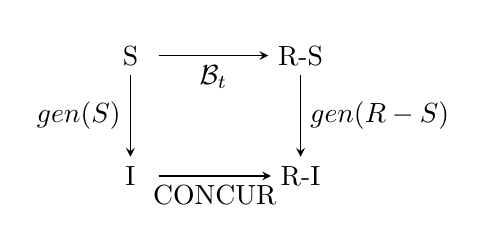
\begin{tikzpicture}
  \matrix (m) [matrix of math nodes,row sep=3em,column sep=4em,minimum width=2em]
  {
    \text{S} & \text{R-S} \\
    \text{I} & \text{R-I} \\};
  \path[-stealth]
  (m-1-1) edge node [left] {$gen(S)$} (m-2-1)
  edge node [below] {$\mathcal{B}_t$} (m-1-2)
  (m-2-1.east|-m-2-2) edge node [below] {$\text{CONCUR}$}
  node [] {} (m-2-2)
  (m-1-2) edge node [right] {$gen(R-S)$} (m-2-2);
\end{tikzpicture}


Rules have the following shape:
\[r: t\rightarrow t'~\text{if}~\overline{eq}_n\]
where $\overline{eq}_n$ is a sequence of equational conditions that we use to
define which transitions are possible and which are not.

Rules are defined by using variables so that with a finite amount of rules we
can capture infinite possible scenarios.

Now we proceed to show how concrete instances can be generated starting from the
schemas. First some notation.

\begin{definition}[Ground Terms]
  For a given signature $\Sigma=\langle Sorts, Operations \rangle$ the set of ground
  terms $T_\Sigma$ is inductively defined as follows:
  \begin{enumerate}
  \item All constants of sorts S in Operations are ground terms of sort S.
  \item For every function symbol $f:S_1,\ldots,S_n\rightarrow S$ in Operations,
    if $t_1,\ldots,t_n$ are ground terms of sorts $S_1,\ldots,S_n$,
    respectively, then $f(t_1,\ldots,t_n)$ is a ground term of sort $S$ where
    $S_1,\ldots,S_n\in Sorts$
  \end{enumerate}

  With $T_\Sigma^n$ we indicate all the ground terms up to the $n$-nth iteration
  of the inductive definition. For example, $T_\Sigma^0$ is the set of constant
  symbols, $T_\Sigma^1$ is the set of ground terms given by all the possible
  applications of the operators to $T_\Sigma^0$, and so on.\\
  With $T_{\Sigma, S}^n$ we indicate the ground terms of sort $S$ up to the
  $n$-nth iteration.
\end{definition}

\begin{algorithm}
  \caption{getInstances($\Sigma,r,E,n$)}\label{alg:cap}
  \begin{algorithmic}
    \State $\langle Sorts, Operators \rangle \gets \Sigma$
    \State $V \gets vars(r)$    \Comment{Get vars used by the rule}
    \State $S = \{\{v\} \times T_{\Sigma,type(v)}^n | v \in V\}$ 
    \State $ConcInst = S_{v_1} \times \ldots \times S_{v_m}$
    \State $ConcRules \gets \emptyset$ 
    \ForEach{$i \in ConcInst$}
    \State $CR \gets instantiate(i,r)$
    \State $t' \rightarrow t'~\text{if}~\overline{eq}_l \gets CR$
    \If{$E\vdash \overline{eq}_l$}
    \State $ConcRules \gets ConcRules \cup \{t \rightarrow t'\}$
    \EndIf
    \EndFor\\
    \Return $ConcRules \cup getInstances(\Sigma,r,E,n+1)$
  \end{algorithmic}
\end{algorithm}

\end{document}